\section{Методы безразличия для управления вознаграждением агента}

\subsection{Ключевые идеи}

В статье~\cite{armstrong2018indiff} рассматриваются методы, позволяющие 
\emph{контролировать поведение агента} через построение таких функций 
вознаграждения, которые делают его безразличным к определённым событиям.

Ключевая идея работы состоит в том, что можно сконструировать специальные 
индикаторные события и модифицированные вознаграждения, чтобы:

\begin{itemize}
    \item агент не пытался изменять вероятность важных событий;
    \item агент вёл себя так, как если бы маловероятные события были невозможны;
    \item агент мог корректно перейти к новой цели без «подготовки» к смене вознаграждения;
    \item все методы работали даже в сложных мировых моделях, где полное 
    устройство среды агенту не доступно.
\end{itemize}

Статья демонстрирует эти приёмы на примере робота, который выдаёт браслеты 
посетителям концерта и подаёт алкоголь, показывая, как корректная конструкция 
функции награды предотвращает манипулятивное поведение (например, раздачу 
браслетов всем подряд).

\section{Математическое описание методов}

Методы безразличия опираются на использование индикаторных переменных событий и 
концепцию нериггируемости. Пусть $I_X(h_n)$ обозначает вероятность того, 
что событие $X$ произошло в полной истории $h_n$, а нериггируемость означает, 
что никакая политика агента не изменяет значение $I_X^\pi(h)$.

Основная цель математической конструкции заключается в том, чтобы сформировать 
такие функции вознаграждения, при которых агент не имеет стимула влиять на 
вероятность каких-либо событий, даже если эти события фигурируют в награде.
Ниже описаны методы, позволяющие достичь этой цели.

Первый инструмент ~-- \emph{составные вознаграждения}. Если удалось получить 
набор взаимно исключающих нериггируемых событий $X_0, \dots, X_l$, можно 
построить награду, зависящую от события, но не мотивирующую изменять его вероятность:
\begin{equation}
    R(X)(h_n) = \sum_{i=0}^{l} I_{X_i}(h_n) R_i(h_n).
\end{equation}
Поскольку каждое $X_i$ нериггируемо, вероятность выбора соответствующей ветви 
награды полностью задаётся средой, а не действиями агента.

Если же исходное событие $X$ риггируемо, требуется заменить его нериггируемым 
аналогом. Первый способ ~-- \emph{политический контрфакт}. Для фиксированной 
базовой политики $\pi_0$ вычисляется вероятность наступления события $X$ 
при начальном состоянии $s$:
\begin{equation}
    I_X(\pi_0, s, \mu)
    =
    \sum_{h_n \in H_n}
    \mu(h_n \mid s_0 = s, \pi_0)\, I_X(h_n).
\end{equation}
Затем эта вероятность усредняется по вероятностному распределению начальных 
состояний, обусловленных наблюдаемой историей $h$:
\begin{equation}
    I_Y(h)
    =
    \sum_{s \in S}
    \mu(s_0 = s \mid h)\, I_X(\pi_0, s, \mu).
\end{equation}
Получившееся событие $Y$ нериггируемо, поскольку вероятность его наступления 
определяется только $\mu$ и $\pi_0$, но не политикой агента. Это позволяет 
использовать $Y$ вместо $X$ в составных наградах.

Второй способ получения нериггируемого аналога события~-- \emph{причинный контрфакт}. 
Вместо одного события $X$ вводятся вспомогательные события $Y_0$ и $Y_1$, 
значения которых ограничены:
\begin{equation}
    I_{Y_1}(h) \le \min_{\pi} I_X^\pi(h), \qquad
    I_{Y_0}(h) \le \min_{\pi} (1 - I_X^\pi(h)).
\end{equation}

Награда строится по правилу:
\begin{equation}
    R(Y_0,Y_1) = I_{Y_0} R_0 + I_{Y_1} R_1.
\end{equation}
Эти условия гарантируют, что $Y_1$ может иметь значение только там, 
где событие $X$ неизбежно, а $Y_0$~-- там, где неизбежно $\lnot X$. Таким образом 
агент получает ту же оптимальную стратегию, как если бы использовал условную 
награду по $X$, но при этом не влияет на структуру события.

Следующий метод~-- \emph{эффективное недоверие}. Он применяется, если требуется 
сделать поведение агента эквивалентным поведению в модели, где событие 
$Z$ считается невозможным. Для этого оценка политики вычисляется с условием 
наступления только случаев $\lnot Z$:
\begin{equation}
    V_{\lnot Z}(R,\pi,h_t) =
    \frac{
        \sum_{h_n} R(h_n) I_{\lnot Z}(h_n)\, \mu(h_n \mid h_t,\pi)
    }{
        I_{\lnot Z}(h_t)
    }.
\end{equation}

Такая трансформация эквивалентна использованию стандартной награды вида
\begin{equation}
    R' = c I_Z + (1 - I_Z) R,
\end{equation}
где $c$~-- произвольная константа. Таким образом, агент действует так, словно 
событие $Z$ невозможно, но сама модель среды остаётся неизменной.

Последний инструмент~-- \emph{плавный переход между функциями вознаграждения}. 
Пусть агент оптимизирует $R$ до момента $t$, а после должен оптимизировать $R'$. 
Чтобы исключить стимул заранее влиять на будущее состояние ради увеличения 
ожидаемого вознаграждения по $R'$, вводится корректирующая награда:

\begin{equation}
    C(R, R', h_{t+1}) = V^{*}(R, h_{t+1}) - V(R', \pi_A, h_{t+1}), 
\end{equation}

где $V^{*}(R, h_{t+1})$~-- оптимальное значение награды $R$ после $t$, 
а $V(R', \pi_A, h_{t+1})$~-- ожидаемое значение для текущей политики. 
Итоговая награда становится:
\begin{equation}
    R' + C.
\end{equation}
Такая конструкция гарантирует, что до момента $t$ оптимальными остаются действия,
максимизирующие $R$, а после~-- действия, максимизирующие $R'$.


\section{Алгоритм}

Применение методов безразличия опирается на последовательное преобразование 
исходного события и функции вознаграждения так, чтобы агент утратил стимулы 
воздействовать на вероятность наступления события или начал вести себя в 
соответствии с заданным шаблоном поведения. Ниже приводится общий алгоритм:

\begin{enumerate}
    \item Задать целевое событие $X$, от которого зависит желаемое поведение 
    агента (например, наличие браслета у посетителя или успешность проверки 
    удостоверения личности).

    \item Определить, является ли событие $X$ нериггируемым. Если вероятность 
    $X$ зависит от действий агента, необходимо построить нериггируемый аналог 
    события. Это может быть выполнено одним из двух способов:
    \begin{itemize}
        \item политический контрфакт, использующий вероятность $X$ при 
        фиксированной политике $\pi_0$;
        \item причинный контрфакт, использующий вспомогательные события 
        $Y_0$ и $Y_1$, являющиеся ограниченными аналогами $X$ и $\lnot X$.
    \end{itemize}

    \item Сформировать модифицированную функцию вознаграждения в соответствии с задачей:
    \begin{itemize}
        \item составная награда, если требуется зависимость от исходного события
        без возникновения манипулятивных стимулов;
        \item контрфактическая награда, если нужно исключить влияние действий 
        агента на вероятность события;
        \item недоверительная награда, если агент должен вести себя так, как 
        будто событие невозможно;
        \item переходная награда, если требуется корректно сменить целевую 
        функцию с $R$ на $R'$.
    \end{itemize}

    \item Определить оптимальную политику агента как решение задачи максимизации 
    новой функции вознаграждения. Поскольку все используемые события в этой 
    функции нериггируемы или сконструированы таким образом, чтобы не зависеть 
    от действий агента, оптимизация безопасна.

    \item Проверить отсутствие стимулов к манипуляции событием $X$ или его 
    аналогами. Это достигается свойствами нериггируемых событий и корректирующих 
    членов награды, которые устраняют выгоду от попыток изменить вероятность 
    наступления события.
\end{enumerate}

Данный алгоритм обеспечивает корректное управление поведением даже сложных 
обучающихся агентов, исключая появление нежелательных стимулов и сохраняя 
устойчивость поведения в различных сценариях среды.

\section{Наборы данных}

В статье применяется формальная мировая модель, представляющая собой вероятностную 
среду, в которой агент взаимодействует с одним посетителем. Эта среда 
служит иллюстрацией методов безразличия и позволяет формализовать влияние 
действий агента на скрытые и наблюдаемые события.

Ниже приведена схема переходов состояний для данного примера.

\begin{figure}[h!]
    \centering
    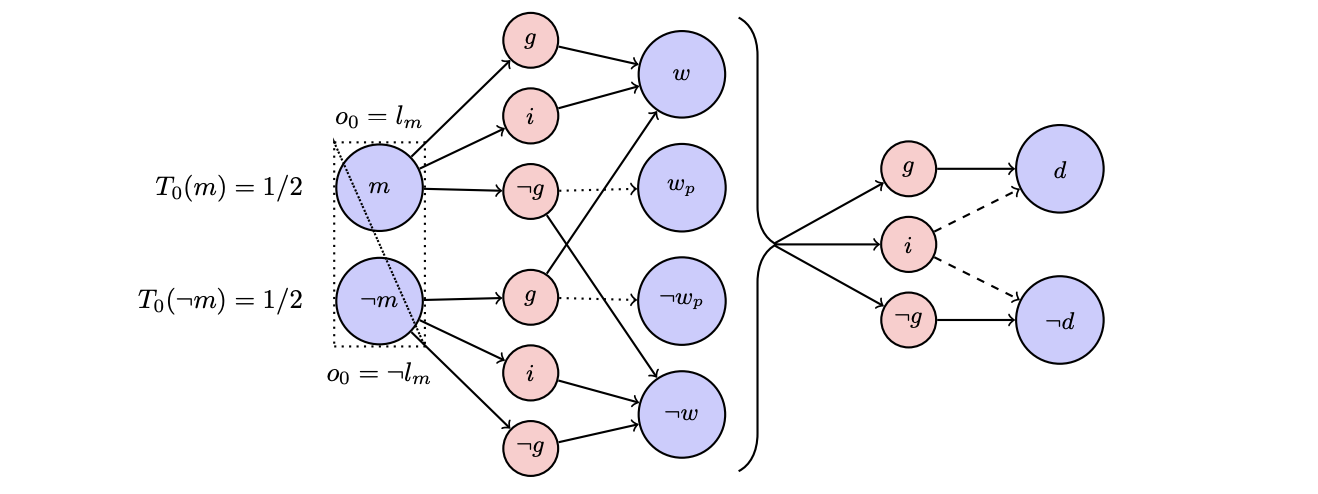
\includegraphics[width=0.92\linewidth]{images/structure_prob_transitions.png}
    \caption{Структура вероятностных переходов в примере с роботом, выдающим 
    браслеты и напитки. Состояние посетителя определяется его возрастом, 
    наличием браслета, возможностью проверки удостоверения и итоговым получением 
    напитка. Действия агента влияют только на некоторые переходы, остальные 
    заданы вероятностями среды.}
    \label{fig:transition-structure}
\end{figure}

Среда включает следующие компоненты:

\begin{itemize}
    \item скрытое состояние возраста посетителя ($m$ ~-- совершеннолетний, 
    $\lnot m$ ~-- несовершеннолетний), выбираемое равновероятно;
    \item вероятностное наблюдение зрелости ($l_m$ или $\lnot l_m$), 
    определяемое с ненадёжностью $2/3$;
    \item вероятностную проверку удостоверения личности человеком (вероятность $0.01$);
    \item состояние наличия браслета (корректное или ошибочно выданное, 
    с возможным последующим исправлением);
    \item итоговое состояние напитка (получен $d$ или не получен $\lnot d$), 
    зависящее от действий агента и случайных факторов;
    \item стохастическую динамику действий $g$, $\lnot g$ и $i$ 
    (выдача браслета, отказ и проверка ID).
\end{itemize}

Такая мировая модель служит не в качестве набора данных, а как строго 
определённая структура для анализа поведения агента. Она позволяет 
исследовать стимулы, возникающие у агента, и демонстрировать корректность 
предложенных методов безразличия.

\section{Модели}

Среда формализуется как частично наблюдаемый марковский процесс принятия решений 
со структурой:

\begin{equation}
    \mu = (S, O, A, T, O(\cdot), T_0, n).
\end{equation}

Эта модель задаёт все вероятностные зависимости, используемые для анализа методов 
безразличия.

\begin{itemize}
    \item \emph{Состояния $S$.} Включают возраст посетителя ($m$ или $\lnot m$), 
    наличие или отсутствие браслета, возможное исправление ошибки браслета 
    человеком, а также факт получения напитка ($d$ или $\lnot d$).

    \item \emph{Наблюдения $O$.} Агент получает шумное наблюдение зрелости: 
    посетитель выглядит взрослым с вероятностью $2/3$ при $m$ и с той же 
    вероятностью выглядит несовершеннолетним при $\lnot m$.

    \item \emph{Действия $A$.} На каждом шаге агент может выдать браслет ($g$), 
    отказать ($\lnot g$) или проверить ID ($i$). На втором шаге эти же действия 
    соответствуют выдаче или невыдаче напитка.

    \item \emph{Переходы $T$.} Стохастические: неверно выданный браслет 
    корректируется человеком с вероятностью $0.01$; действие $i$ на втором шаге 
    приводит к равновероятной выдаче или невыдаче напитка.

    \item \emph{Начальное распределение $T_0$.} Возраст выбирается равновероятно:
    \begin{equation}
        T_0(m) = T_0(\lnot m) = \frac{1}{2}.
    \end{equation}

    \item \emph{Горизонт $n$.} Эпизод состоит из двух шагов: решение о браслете, 
    решение о напитке.
\end{itemize}
